\chapter{Evaluation der Anwendung}\label{chapter_6}
Die Anwendung wurde anhand der spezifizierten Anforderungen in Kapitel \ref{requirements} umgesetzt. Beim Entwurf der Ansichten sind die Heuristiken von Nielsen, sowie die Designrichtlinien von Microsoft für die Zielplattform verwendet worden. Eine Überprüfung, ob die Ziele, die zuvor gestellt wurden erreicht sind, wird mithilfe einer Evaluation der Anwendung sichergestellt. Der Aufbau und die Zielsetzung wird im Folgenden beschrieben. 

\section{Durchführung der Evaluation}
Der neue Workflow, wie in Kapitel \ref{chapter_3} beschrieben, ist auf die Verwendung mit einem mobilen Endgerät zugeschnitten. Aus diesem Grund ist eine Evaluation des Gesamtprozesses nicht zielführend. Wichtiger ist die Erfüllung der gestellten Anforderungen. Wenn diese erfüllt sind, so kann der modellierte Prozess umgesetzt werden. Für die Untersuchung der verschiedenen Anforderungstypen werden unterschiedliche Evaluationen durchgeführt.

\subsection{Funktionale Anforderungen}
Die Funktionalen Anforderungen aus Abschnitt \ref{functionRequ} werden mit Anwendern überprüft. Hierzu wird die alte Weboberfläche, die für die Konfiguration zuständig ist, als Ausgangspunkt verwendet. Da in der neuen Anwendung ein zusätzlicher Produktkatalog integriert ist, wird kein direkter Vergleich der beiden Lösungen durchgeführt. Stattdessen werden gezielte Aufgaben an die Benutzer gestellt, die eine Umsetzung der Anforderungen überprüft. Die einzelnen Aufgabenstellungen werden anhand einer Skala von 1-5 bewertet. Bei der Bewertung wird die Frage, wie gut oder schlecht die Aufgabe durchgeführt werden kann, für eine Bewertungsgrundlage verwendet. 

Da die aktuelle Konfigurationslösung für Experten entwickelt wurde, wird die Benutzerevaluation in einer Interview Form durchgeführt. Die auftretenden Fragen werden protokolliert, so dass auftretende Probleme besser erkannt werden können. 

\subsection{Nicht-Funktionale Anforderungen}
Eine Überprüfung der Nicht-Funktionalen Anforderungen ist eine größere Herausforderung, da hier meist subjektive Meinungen entstehen. Aus diesem Grund wurde bei der Spezifikation der Anforderungen die zehn Heuristiken von Nielson verwendet. Anhand dieser kann eine Auswertung der Anwendung erfolgen. Hierzu werden zwei unterschiedliche Arten von Tests durchgeführt. Die zuvor genannten Benutzertests werden mit zusätzlichen Fragen zur Verwendung der App erweitert. Die Fragestellungen beziehen sich auf eine subjektive Wahrnehmung der Nicht-Funktionalen Anforderungen. Für eine objektivere Sicht wird eine zusätzliche Expertenevaluation durchgeführt, bei der die zehn Heuristiken von Nielsen bewertet werden. Die Experten kennen sich mit dem System, sowie mit Benutzerschnittstellen aus und können so gezielt die Eigenschaften des Systems untersuchen. Bei der Durchführung wird der Experte die Anwendung ohne Vorgaben überprüfen und anschließend eine Bewertung anhand der vorgegebenen Kriterien abgeben. 

\subsection{Auswahl der Testmenge}
Damit eine Evaluation sinnvoll ist, muss eine geeignete Anzahl von Testergebnissen vorliegen. Anhand der Untersuchungen von Nielsen \cite{bib:countTests} findet eine Anzahl von fünf Personen bereits 75\% aller Usability Probleme. Weiterhin hat eine Anzahl von drei Benutzern das beste Verhältnis von Kosten und Nutzen. Aus diesem Grund werden vier Benutzertests und drei Expertentests durchgeführt. 

\section{Ergebnisse}

\subsection{Allgemeine Auswertung}
\subsection{Benutzerauswertung}
\begin{figure}
\centering
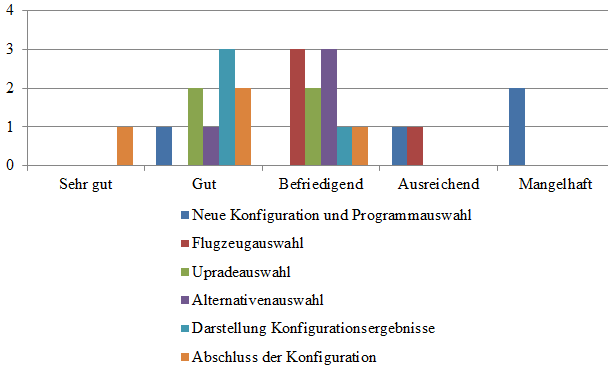
\includegraphics[width=\hsize]{images/bewertung_webgui}
\caption{Komponenten im MVVM Entwurfsmuster}
\label{bewertungWebgui}
\end{figure}
\begin{figure}
\centering
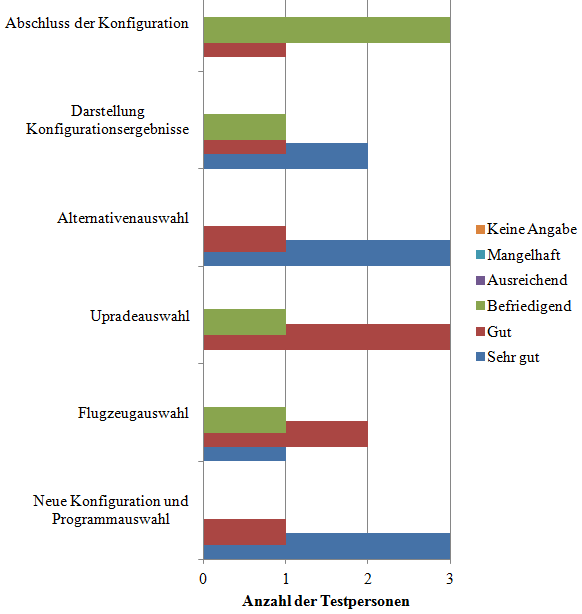
\includegraphics[width=\hsize]{images/bewertung_tablet}
\caption{Komponenten im MVVM Entwurfsmuster}
\label{bewertungTablet}
\end{figure}
\begin{figure}
\centering
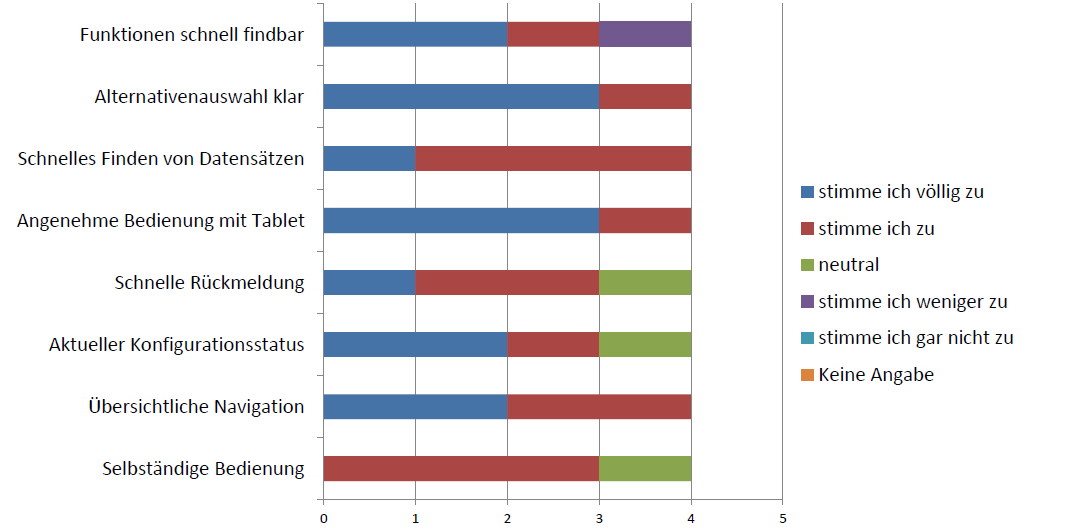
\includegraphics[width=\hsize]{images/bewertung_ux}
\caption{Komponenten im MVVM Entwurfsmuster}
\label{bewertungUx}
\end{figure}
\subsection{Expertenauswertung}

\section{Anpassungen an die Zusammenfassung}